% Figura cuerpo B2 (3.1.2): la rigidez real como amplificador: cuanto menos se mueve el precio deseado, más muerde la fricción nominal
\documentclass[tikz,border=3pt]{standalone}
\usepackage[T1]{fontenc}
\usepackage[utf8]{inputenc}
\usepackage{amsmath}
\usetikzlibrary{arrows.meta,calc,positioning}
\begin{document}
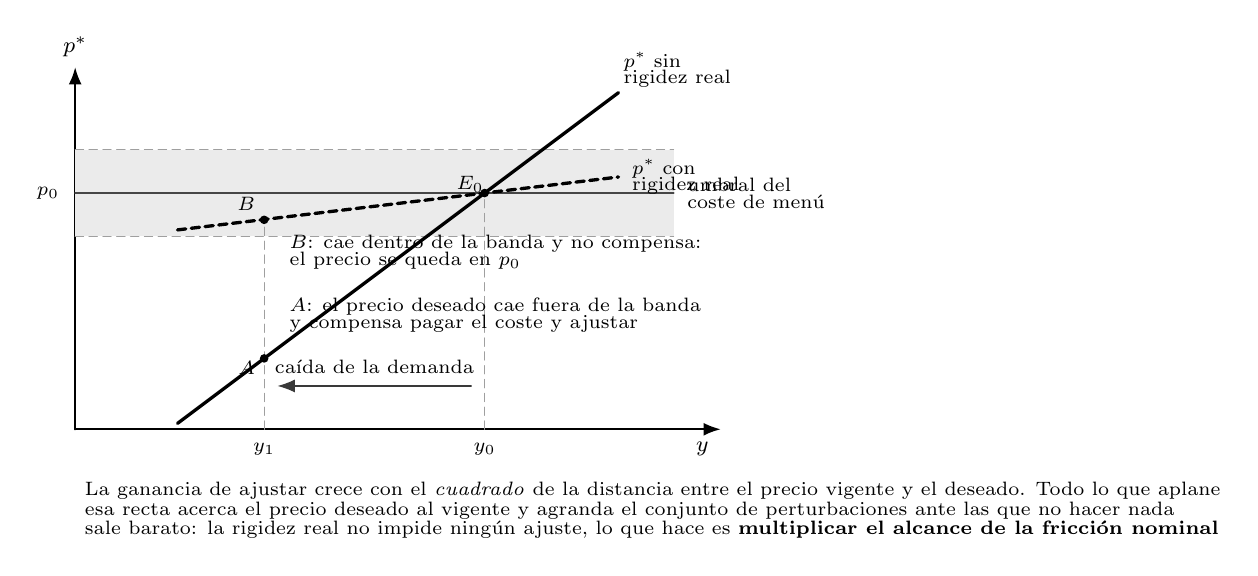
\begin{tikzpicture}[>={Latex[length=2.2mm]}, line cap=round, font=\footnotesize,
  eje/.style={->, thick},
  curva/.style={very thick},
  plana/.style={very thick, densely dashed},
  guia/.style={densely dashed, gray!75},
  pto/.style={circle, fill=black, inner sep=1.1pt}]

  \draw[eje] (0,0) -- (8.2,0) node[below left=1pt]{$y$};
  \draw[eje] (0,0) -- (0,4.6) node[above]{$p^{*}$};

  % Banda del umbral del coste de menú alrededor del precio vigente
  \fill[black!8] (0,2.45) rectangle (7.6,3.55);
  \draw[guia] (0,2.45) -- (7.6,2.45);
  \draw[guia] (0,3.55) -- (7.6,3.55);
  \node[anchor=west, font=\scriptsize, align=left] at (7.65,3.0)
    {umbral del\\[-2pt]coste de menú};

  % Precio vigente
  \draw[thick, gray!55!black] (0,3.0) -- (7.6,3.0);
  \node[anchor=east, font=\scriptsize] at (-0.08,3.0) {$p_{0}$};

  % Precio deseado: sin rigidez real (pendiente grande) y con ella (pendiente pequeña)
  \draw[curva] (1.3,0.075) -- (6.9,4.275) node[above right=-3pt, font=\scriptsize, align=left]{$p^{*}$ sin\\[-2pt]rigidez real};
  \draw[plana] (1.3,2.532) -- (6.9,3.204) node[right=1pt, font=\scriptsize, align=left]{$p^{*}$ con\\[-2pt]rigidez real};

  % Caída de la demanda
  \draw[guia] (5.2,0) -- (5.2,3.0);
  \draw[guia] (2.4,0) -- (2.4,2.66);
  \node[below, font=\scriptsize] at (5.2,-0.05) {$y_{0}$};
  \node[below, font=\scriptsize] at (2.4,-0.05) {$y_{1}$};
  \draw[<-, gray!45!black, shorten >=2pt, shorten <=2pt] (2.5,0.55) -- (5.1,0.55);
  \node[font=\scriptsize, anchor=south] at (3.8,0.58) {caída de la demanda};

  \node[pto] (E0) at (5.2,3.0) {};
  \node[above left=-3pt of E0, inner sep=1pt, font=\scriptsize] {$E_{0}$};
  \node[pto] (A) at (2.4,0.9) {};
  \node[anchor=north east, inner sep=2pt, font=\scriptsize] at (2.36,0.94) {$A$};
  \node[pto] (B) at (2.4,2.66) {};
  \node[anchor=south east, inner sep=2pt, font=\scriptsize] at (2.36,2.70) {$B$};

  \node[anchor=west, font=\scriptsize, align=left] at (2.6,1.45)
    {$A$: el precio deseado cae fuera de la banda\\[-2pt]y compensa pagar el coste y ajustar};
  \node[anchor=west, font=\scriptsize, align=left] at (2.6,2.25)
    {$B$: cae dentro de la banda y no compensa:\\[-2pt]el precio se queda en $p_{0}$};

  \node[align=left, anchor=north west, font=\scriptsize] at (0,-0.55)
    {La ganancia de ajustar crece con el \textit{cuadrado} de la distancia entre el precio vigente y el deseado. Todo lo que aplane\\[-1pt]esa recta acerca el precio deseado al vigente y agranda el conjunto de perturbaciones ante las que no hacer nada\\[-1pt]sale barato: la rigidez real no impide ningún ajuste, lo que hace es \textbf{multiplicar el alcance de la fricción nominal}};
\end{tikzpicture}
\end{document}
